\chapter{Avaliação empírica}


A fim de realizar a validação da ideia do ModMan, o capítulo corrente aborda a prova de conceito do sistema e é composto por cinco seções. A Seção \ref{prova} traz os elementos sobre a prova de conceito, a Seção \ref{questionario} traz o questionário aplicado às pessoas que testarem o sistema e a Seção \ref{avaliacoes} discorre sobre as avaliações que foram realizadas. A Seção \ref{consideracoes} apresenta algumas considerações relevantes sobre a avaliação realizada. Por fim, a Seção \ref{ameacas} traz as possibilidades que podem influenciar negativamente na validação da proposta.


\section{Prova de conceito}\label{prova}


A prova de conceito, tradução do conhecido termo em inglês PoC (Proof of Concept) é utilizado para desenvolver na prática, artefatos que possam mostrar o funcionamento de alguma coisa que ainda se encontre em fase teórica. Segundo Basili \citep{Basili1991}, a definição de \textit{prova de conceito} pode ser resumida como um estudo pequeno em que finalidade é a validação da funcionalidade da aplicação da nova ideia. Além disso, a definição do estudo piloto pode ser resumida como um pequeno estudo desenvolvido após o estudo de prova de conceito, e cujo objetivo é elaborar e provar uma protótipo de solução final em um pequeno caso real.
Desta forma, a prova de conceito será utilizada para obter artefatos de softwaes que possam comprovar que o trabalho proposto realmente pode funcionar e, a partir disso, discutir a viabilidade da implementação do mesmo perante outros softwares.

O ModMan pode ser imaginado em diversas situações e por exemplo, é possível integrá-lo junto a um sistema cliente feito em plataforma Desktop, Web ou mobile. Ainda assim, tem a situação do sistema cliente ser um projeto novo ou em andamento. Desta forma, a prova de conceito é aplicada testando a viabilidade em distintos cenários buscando embasar o funcionamento.

Neste trabalho, a prova de conceito busca por meio de dois desenvolvedores, construir aplicações que consumam a API disponibilizada pelo ModMan. Para isso, fica a cargo de cada um, realizar a integração a problemas particulares. A fim de diversificar as provas de conceito, as mesmas contemplaram sistemas Web e aplicativos mobile, alternando em cenários novos e existentes. Em seguida, aplicou-se o questionário da Seção \ref{questionario} buscando obter a percepção dos desenvolvedores quanto ao uso da abordagem proposta.


\section{Questionário}\label{questionario}


Com o objetivo de contextualizar e obter detalhes sobre o teste realizado pelos desenvolvedores, os mesmos responderam a um questionário para fornecer dados sobre a eficácia do trabalho proposto e também sobre as suas características. O questionário foi aplicado após a construção da aplicação que consome o ModMan e a análise possibilitou tecer conclusões pertinentes à abordagem proposta. O questionário é dividido em duas seções: Background, que coleta características pessoais dos testadores e Aspecos da implementação, que coleta dados relevantes de cada teste realizado.

Background:
\begin{itemize}

\item \textbf{Questão 1:} Qual o seu tempo de experiência com desenvolvimento de software?

\textbf{Opções de resposta:} 
\begin{itemize}
\item 1 a 2 anos
\item 3 a 5 anos
\item Mais de 5 anos
\end{itemize}

\item \textbf{Questão 2:} Qual o seu tempo de experiência com desenvolvimento de sistemas Web?

\textbf{Opções de resposta:}
\begin{itemize}
\item 1 a 2 anos
\item 3 a 5 anos
\item Mais de 5 anos
\end{itemize}

\item \textbf{Questão 3:} Experiência com o uso de frameworks Web (prover reuso de software)

\textbf{Opções de resposta:} Escala de 1 a 5 (1=Nenhuma, 5=Expert)

\item \textbf{Questão 4:} Qual(s) framework(s) de desenvolvimento Web você costuma utilizar?

\textbf{Opção de resposta:} Texto curto

\item \textbf{Questão 5:} Em linhas gerais, qual o nível de preocupação das equipes em prover o reuso de software?

\textbf{Opções de resposta:} Escala de 1 a 5 (1=Muito baixo, 5=Muito alto)

\item \textbf{Questão 6:} Você costuma utilizar o módulo de controle de acesso e permissão fornecido pela ferramenta que trabalha ou adota evoluções para um padrão próprio?

\textbf{Opções de resposta:} 
\begin{itemize}
\item Adoto o do framework que trabalho sem alterações
\item Adoto o do framework que trabalho mas costumo realizar melhorias
\item Costumo desenvolver um modelo próprio
\end{itemize}

\item \textbf{Questão 7:} Numa empresa que trabalha com diversas tecnologias de desenvolvimento de software, em qual grau você classifica como desvantagem a adoção de diferentes formas de controle dos módulos e perfis devido à variação das tecnologias?

\textbf{Opções de resposta:}
\begin{itemize}
\item Irrelevante
\item Atrapalha a manutenção mas pode ser mediado sem problema
\item Traz prejuízo para a manutenção
\end{itemize}
\item \textbf{Questão 8:} Em qual grau você classifica a importância de uma empresa padronizar o módulo de permissão de acesso dos sistemas por ela desenvolvidos?

\textbf{Opções de resposta:} Escala de 1 a 5 (1=Muito baixo, 5=Muito alto)

\item \textbf{Questão 9:} Com a disponibilidade de um serviço de controle de permissão de acesso, você migraria sistemas que já estão em produção a fim de padronizar os seus sistemas ?

\textbf{Opções de resposta:} Sim, Depende da complexidade da mudança e Não realizaria esse tipo de mudança num sistema em produção

\item \textbf{Questão 10:} No caso do desenvolvimento de novos sistemas, você adotaria a ferramenta proposta de serviço de permissão de acesso?

\textbf{Opções de resposta:} Sim, Talvez, dependendo da complexidade para aplicar e Não, usaria o modelo da própria ferramenta

\item \textbf{Questão 11:} Você achou a proposta válida? Voltaria a utilizar? Comente a experiência/percepção de uso da abordagem proposta.

\textbf{Opções de resposta:} Texto livre

\end{itemize}

Aspectos da implementação:
\begin{itemize}

\item \textbf{Questão 12:} Quantas linhas de código foram inseridas para implementar o uso do sistema de permissões como serviço?

\textbf{Opções de resposta:} Valor livre

\item \textbf{Questão 13:} E quantas linhas foram alteradas?

\textbf{Opções de resposta:} Valor livre

\item \textbf{Questão 14:} Qual o nível de dificuldade de integração numa escala de 1 a 10 ?

\textbf{Opções de resposta:} Escala de 1 a 10 (1=Muito fácil, 10=Muito difícil)


\end{itemize}


As questões tem aspectos técnicos, para coletar dados específicos relevantes ao processo de construção de um software, a fim de obter conhecimento sobre o impacto da implantação do sistema de permissões proposto. E para avaliar os itens técnicos, também é composto por perguntas que ilustram a experiência do desenvolvedor.


\section{Avaliações}\label{avaliacoes}

Esta seção detalha os testes realizados pelos desenvolvedores para realizar a avaliação e apresenta detalhes sobre a implementação como, por exemplo, as tecnologias utilizadas e o procedimento adotado para realizar a integração.

\subsection{Teste 1}

O teste 1 foi realizado pelo Desenvolvedor A numa aplicação existente do Ionic framework com integração ao Laravel Framework. Trata-se de um aplicativo de acompanhamento escolar e o teste realizado foi aplicado no menu do aplicativo, a fim de avaliar o comportamento do processo de integração com um aplicativo mobile já existente. O código fonte deste projeto não está disponível para consulta, pois trata-se de um projeto privado de uma empresa.
A Figura \ref{fig:print1} mostra o trecho de código que foi necessário ser acrescentado no software existente, de forma a realizar a integração. A responsabilidade deste trecho, é buscar os dados que foram cadastrados no sistema de permissões e organizá-los de maneira que a integração com a interface seja simples. A Figura \ref{fig:print2} mostra como tal integração ocorreu, bastando acrescentar uma verificação nas tags dos itens do menu. O funcionamento da integração do teste 1 ocorreu com sucesso pois as permissões foram devidamente aplicadas.

\begin{figure}
	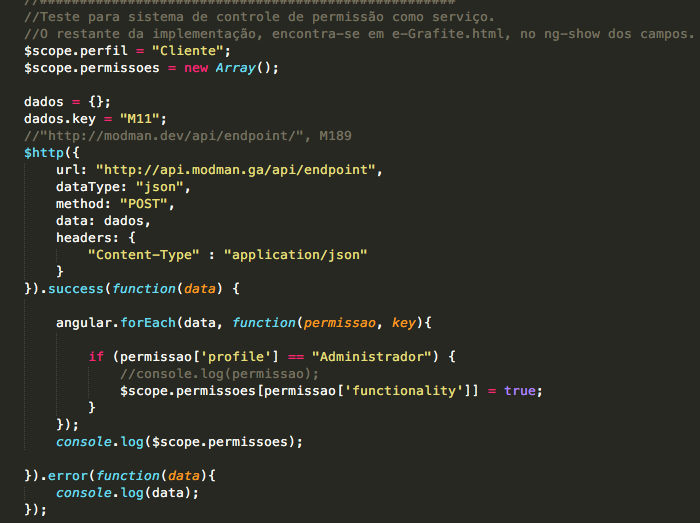
\includegraphics[width=1\textwidth]{images/edic_a_o_do_controller-_teste_do_app_do_e-grafite}
	\caption{Código do controller do teste 1}
    \label{fig:print1}
\end{figure}

\begin{figure}
	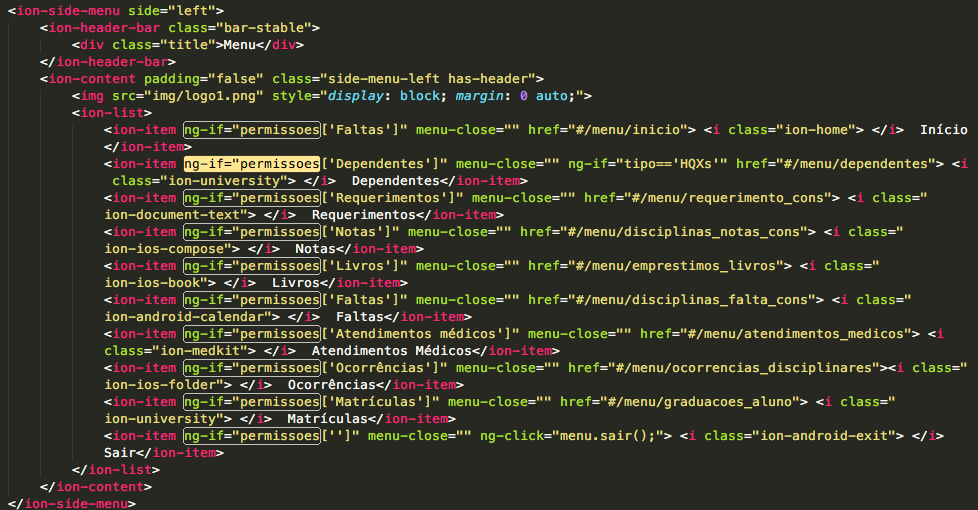
\includegraphics[width=1\textwidth]{images/edic_a_o_da_view_-_teste_do_app_do_e-grafite}
	\caption{Código da view do teste 1}
    \label{fig:print2}
\end{figure}


\subsection{Teste 2}

O teste 2 foi realizado numa nova aplicação Web em PHP desenvolvida exclusivamente para testar o ModMan. O objetivo foi parametrizar a disponibilidade de ações num formulário utilizando somente o Laravel Framework. A aplicação foi desenvolvida pelo mesmo Desenvolvedor A que realizou o Teste 1 e encontra-se disponível no Github no link https://github.com/guiassemany/modman-concept. A Figura \ref{fig:trait} mostra a Trait (Grupo de métodos para incluir em outra classe) CheckPermissionTrait, o qual contém o método hasPermission() que realiza a requisição POST para consultar as permissões. Assim, as classes importam a CheckPermissionTrait, tratando de acordo com a necessidade e aplicam na view, conforme mostrado na Figura \ref{fig:view_laravel}. De acordo com a estrutura adotada, o teste 2 foi executado com sucesso pois as permissões foram devidamente aplicadas.

\begin{figure}
	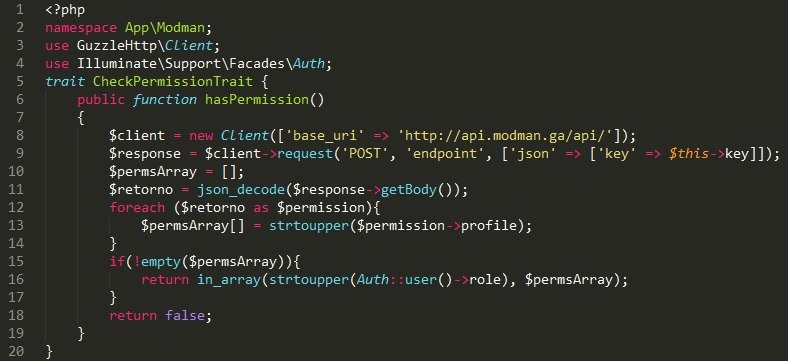
\includegraphics[width=1\textwidth]{images/trait.jpg}
	\caption{Trait desenvolvida no teste 2}
    \label{fig:trait}
\end{figure}

\begin{figure}
	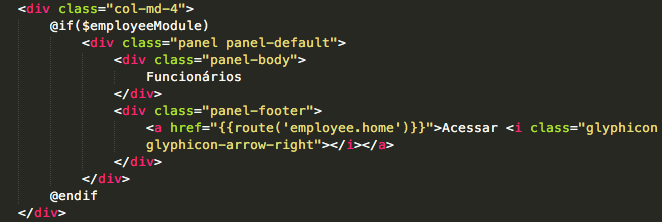
\includegraphics[width=1\textwidth]{images/view_laravel.png}
	\caption{Código da view do teste 2}
    \label{fig:view_laravel}
\end{figure}


\subsection{Teste 3}


O teste 3 foi realizado pelo Desenvolvedor B numa aplicação Web existente, desenvolvida com PHP no back-end e Javascript no front-end com arquitetura de Single page Application, a fim de avaliar o comportamento da integração e possíveis complicação durante o processo. O sistema do teste 3 é de gerenciamento de oficina mecânica e foi desenvolvido com o Laravel Framework e o AngularJs e não contém o código fonte disponível para demonstração por se tratar de um software proprietário. O objetivo do teste foi aplicar as devidas permissões para a dashboard do sistema, representada na Figura \ref{fig:dashboard_oficina} que contém acessos rápidos aos usuários e deve ter os itens disponíveis somente para o funcionário que trata do correspondente setor da oficina. Para realizar a integração, o código da Figura \ref{fig:controller_oficina} trata do back-end, realizando uma requisição POST que envia o devido parâmetro "key", tratando o JSON retornado para utilizá-lo na view, que apenas verifica a disponibilidade da variável da permissão para exibir ou não o determinado item da dashboard. Utilizando a estrutura apresentada, o teste 3 ocorreu com sucesso.


\begin{figure}
	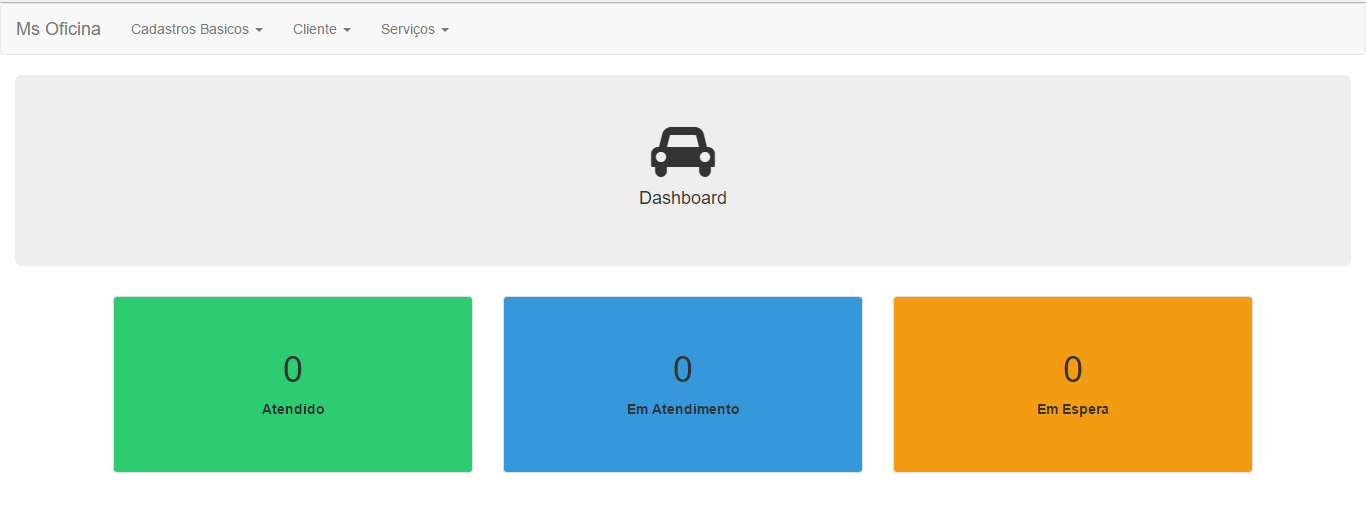
\includegraphics[width=1\textwidth]{images/dash_oficina.png}
	\caption{Dashboard do sistema do teste 3}
    \label{fig:dashboard_oficina}
\end{figure}

\begin{figure}
	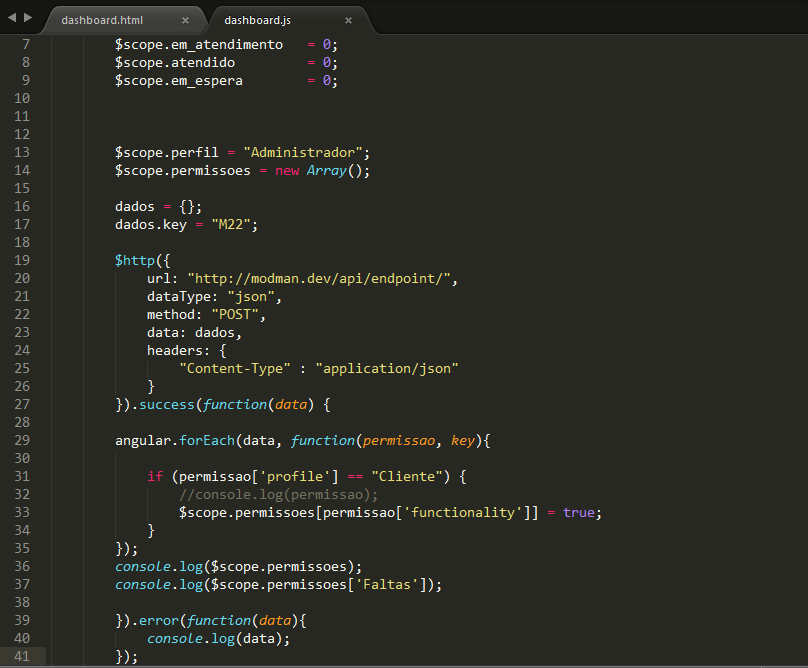
\includegraphics[width=1\textwidth]{images/controller_oficina.png}
	\caption{Controller de integração do teste 3}
    \label{fig:controller_oficina}
\end{figure}


\section{Considerações}\label{consideracoes}


Esta seção traz uma análise sobre as avaliações realizadas discorrendo acerca do questionário que os avaliadores responderam. Para prover a discussão, a Tabela \ref{tabela1} contém as respostas que se referem ao background dos avaliadores e a \ref{tabela2} contém os aspectos da implementação.
Com base nas resposta fornecidas ao formulário é possível notar que os avaliadores têm experiência considerável em tecnologias utilizadas no desenvolvimento Web, o que pode ter colaborado para a integração simples e de baixo impacto, de acordo com as respostas de ambos. A constatação de facilidade na integração do sistema proposto com sistemas clientes é baseada no feedback de edição e acréscimo de poucas linhas de código, e a facilidade ocorreu nos ambientes Web e mobile, o que evidencia a interoperabilidade.

Ambos avaliadores responderam que costumam desenvolver um modelo próprio de permissão nos softwares, o que favorece a adoção deste projeto pois seria possível reduzir este esforço.
De acordo com o resposta do Desenvolvedor A na questão 14, tem-se o feedback de que o integração do projeto é simples e funcional, entretanto, houve a sugestão de possibilitar a ativação/inativação dos cadastros no sistema. Essa sugestão é bastante pertinente pois possibilita maior flexibilidade sem necessidade de codificação, o que facilita a manutenção e abrange mais a possibilidade da administração das permissões por meio de pessoas que não tem conhecimento de desenvolvimento de software.
Os avaliadores responderam que usariam este trabalho, entretanto, vale ressaltar que de acordo com eles, a viabilidade de integração depende da complexidade da mudança no dado contexto, que nem sempre poderá ser favorável como os aqui apresentados.

\begin{center}
  \begin{table}
  \label{tabela1}
  \caption{Respostas fornecidas no formulário - Background}
    \begin{tabular}{| c | p{7cm} | c |}
      \hline
      Questão & Guilherme Assemany (Desenvolvedor A)& Matheus Marques (Desenvolvedor B)\\
      \hline
      1 & Mais de cinco anos & 3 a 5 anos\\ \hline
      2 & Mais de cinco anos & 3 a 5 anos\\ \hline
      3 & 3 & 3\\ \hline
      4 & Laravel, Slim, Angular, React & Laravel\\ \hline
      5 & 4 & 3\\ \hline
      6 & Costumo desenvolver um modelo próprio & Costumo desenvolver um modelo próprio\\ \hline
      7 & Irrelevante & Traz prejuízo para a manutenção\\ \hline
      8 & 5 & 5\\ \hline
      9 & Depende da complexidade da mudança & Depende da complexidade da mudança\\ \hline
      10 & Sim & Sim\\ \hline
      11 & Sim. O projeto proposto é bastante eficiente e verdadeiramente utilizável em aplicações. Além de ser fácil de implementar, dá uma possibilidade de enxergar um sistema de forma mais modular e ter mais controle sob suas funcionalidades. Como uma melhoria, seria bom se houvesse algum marcador de ativo / inativo no gerenciamento das regras dos módulos e das funcionalidades, dessa forma seria mais agradável para o utilizar controlar o status de cada pequena parte do sistema.
 & Sem resposta\\ \hline
    \end{tabular}
  \end{table}
\end{center}

\begin{center}
  \begin{table}
  \label{tabela2}
  \caption{Respostas fornecidas no formulário - Referente à implementação}
    \begin{tabular}{| c | p{5cm} | p{4cm} | p{4cm} |}
      \hline
      Questão & Teste 1& Teste 2 & Teste 3\\
      \hline
	  12 & 40 a 60 & 22 & 30\\ \hline
      13 & 5 & 3 & 4\\ \hline
      14 & 2 & 4 & 3\\ \hline
\end{tabular}
  \end{table}
\end{center}

\section{Ameaças}\label{ameacas}  	%http://universalteacher.com/1/threats-to-validity-in-qualitative-research/


Conforme apresentado na prova de conceito do presente capítulo, este trabalho mostrou-se viável.
Entretanto, é importante citar que apesar da obtenção do sucesso na integração, alguns fatores podem ter influenciado para o sucesso. Dentre esses fatores, cita-se a realização da avaliação com softwares pequenos e de arquitetura semelhante, o que deixa em aberto a análise de viabilidade em sistemas de maior porte. 
O mesmo vale para a arquitetura do software cliente, pois é possível integrar com diversas linguagens, inclusive de plataforma Desktop, mas não foram desenvolvidas provas para esses cenários.
Também, os avaliadores detém forte conhecimento no contexto, o que naturalmente tornou o procedimento descomplidado. Possivelmente, um programador que não tem experiência sólida no desenvolvimento Web encontre dificuldade na integração e aponte deficiências ainda não detectadas.
